\documentclass{standalone}
\usepackage{tikz}


\begin{document}
        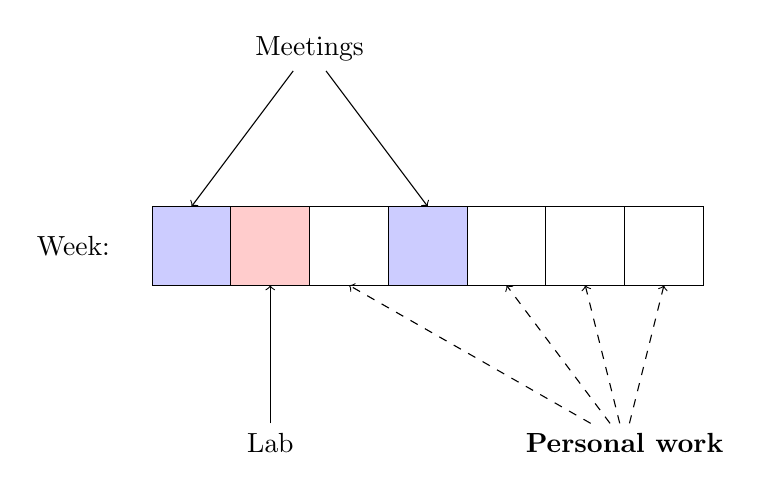
\begin{tikzpicture}
            \node at (-1, .5) {Week:};
            \draw (0, 0)  rectangle  (7, 1);

            \foreach \i in {1,...,6}
                {
                    \draw (\i, 0) -- (\i, 1);
                }

            \draw [fill=blue!20] (0, 0) rectangle (1, 1);
            \draw [fill=red!20] (1, 0) rectangle (2, 1);
            \draw [fill=blue!20] (3, 0) rectangle (4, 1);

            \node (class meetings) at (2, 3) {Meetings};

            \foreach \i in {.5, 3.5}
                {
                    \draw [->] (class meetings) -- (\i, 1);
                }

            \node (lab) at (1.5, -2) {Lab};
            \draw [->] (lab) -- (1.5, 0);

            \node (personal work) at (6, -2) {\textbf{Personal work}};
            \foreach \i in {2.5, 4.5, 5.5, 6.5}
                {
                    \draw [dashed, ->] (personal work) -- (\i, 0);
                }
    \end{tikzpicture}
\end{document}
